\chapter{Аналитическая часть}

\section{Реализация алгоритма поиска подстроки в файле}

В листинге \ref{lst:tf_alg} приведена реализация алгоритма поиска подстроки в строках, читаемых из файла.
При нахождении подстроки, в результирующий файл записываются номер строки и столбца первого символа найденной подстроки.

\clearpage

\lstinputlisting[label=lst:tf_alg,caption=Функция поиска подстроки в файле с последующей записью в результирующем файле, firstline=1,lastline=32]{../tf_alg.cpp}

\section{Графовые представления}

На рисунках \ref{fig:g1} -- \ref{fig:g34} показаны граф управления, информационный граф, операционная история и информационная история соответственно.

\begin{figure}[h]
	\centering
	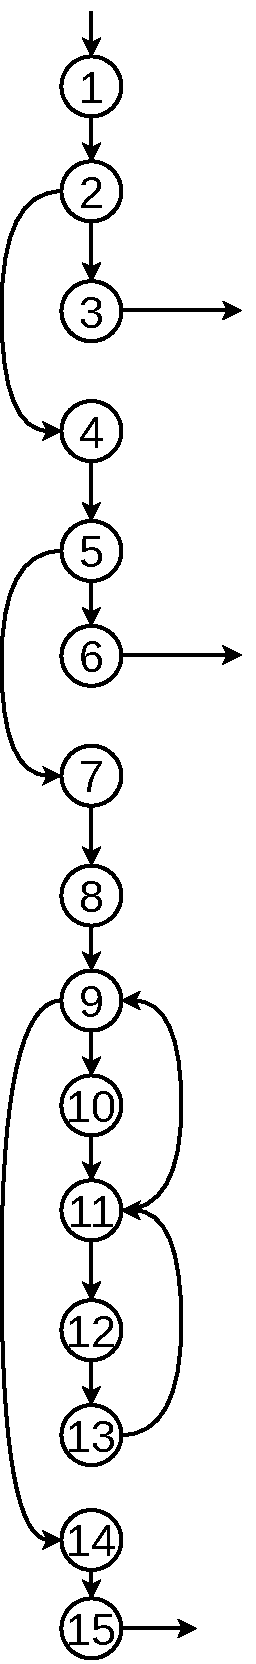
\includegraphics[height=0.9\textheight]{img/ГУ.pdf}
	\caption{Операционный граф}
	\label{fig:g1}
\end{figure}

\begin{figure}[h]
	\centering
	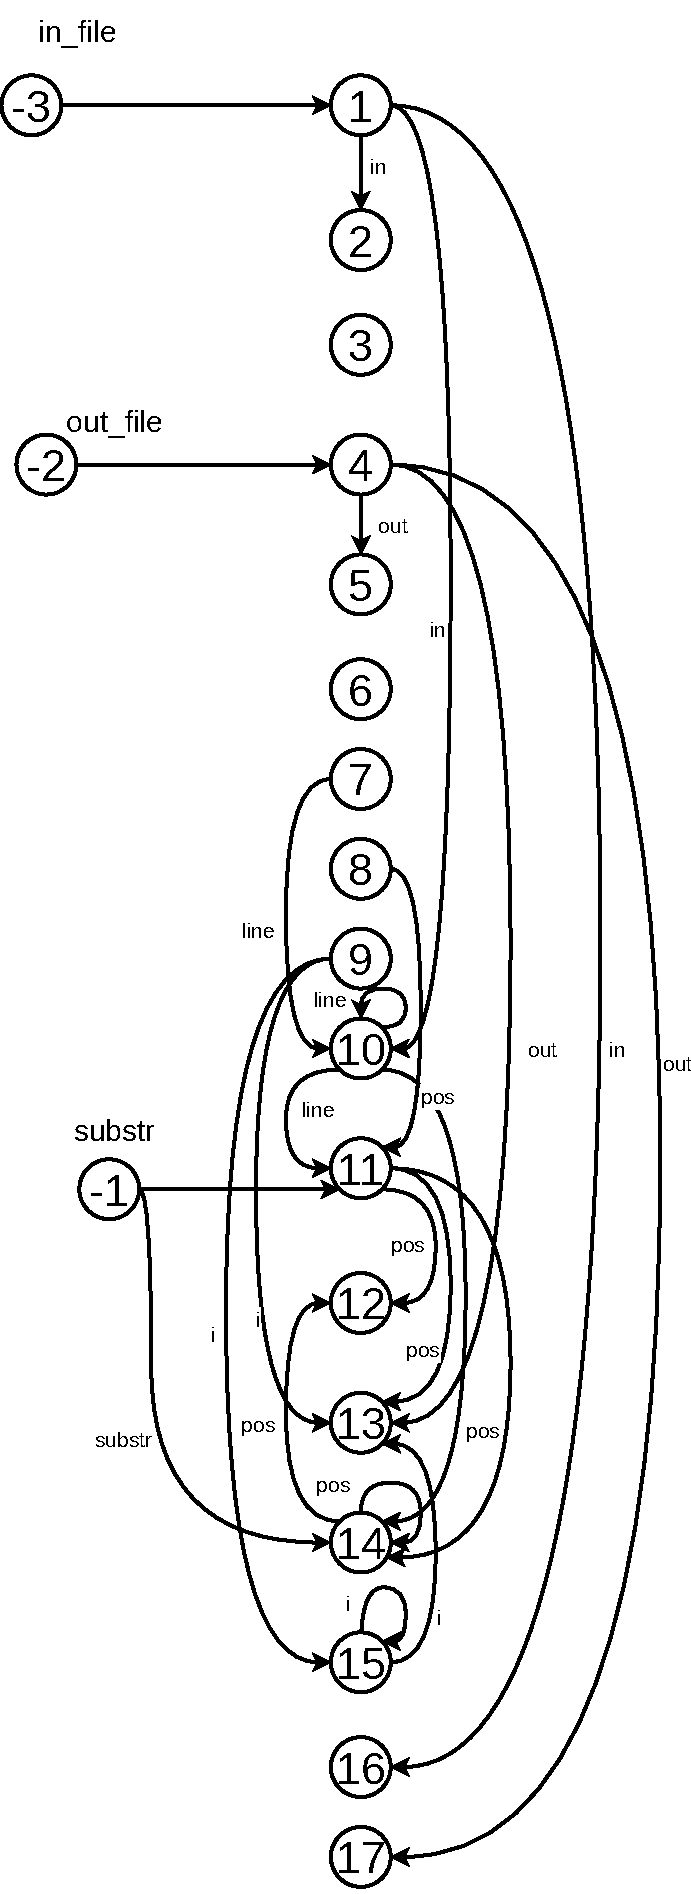
\includegraphics[height=0.9\textheight]{img/ИГ.pdf}
	\caption{Информационный граф}
	\label{fig:g2}
\end{figure}

\begin{figure}[h]
	\centering
	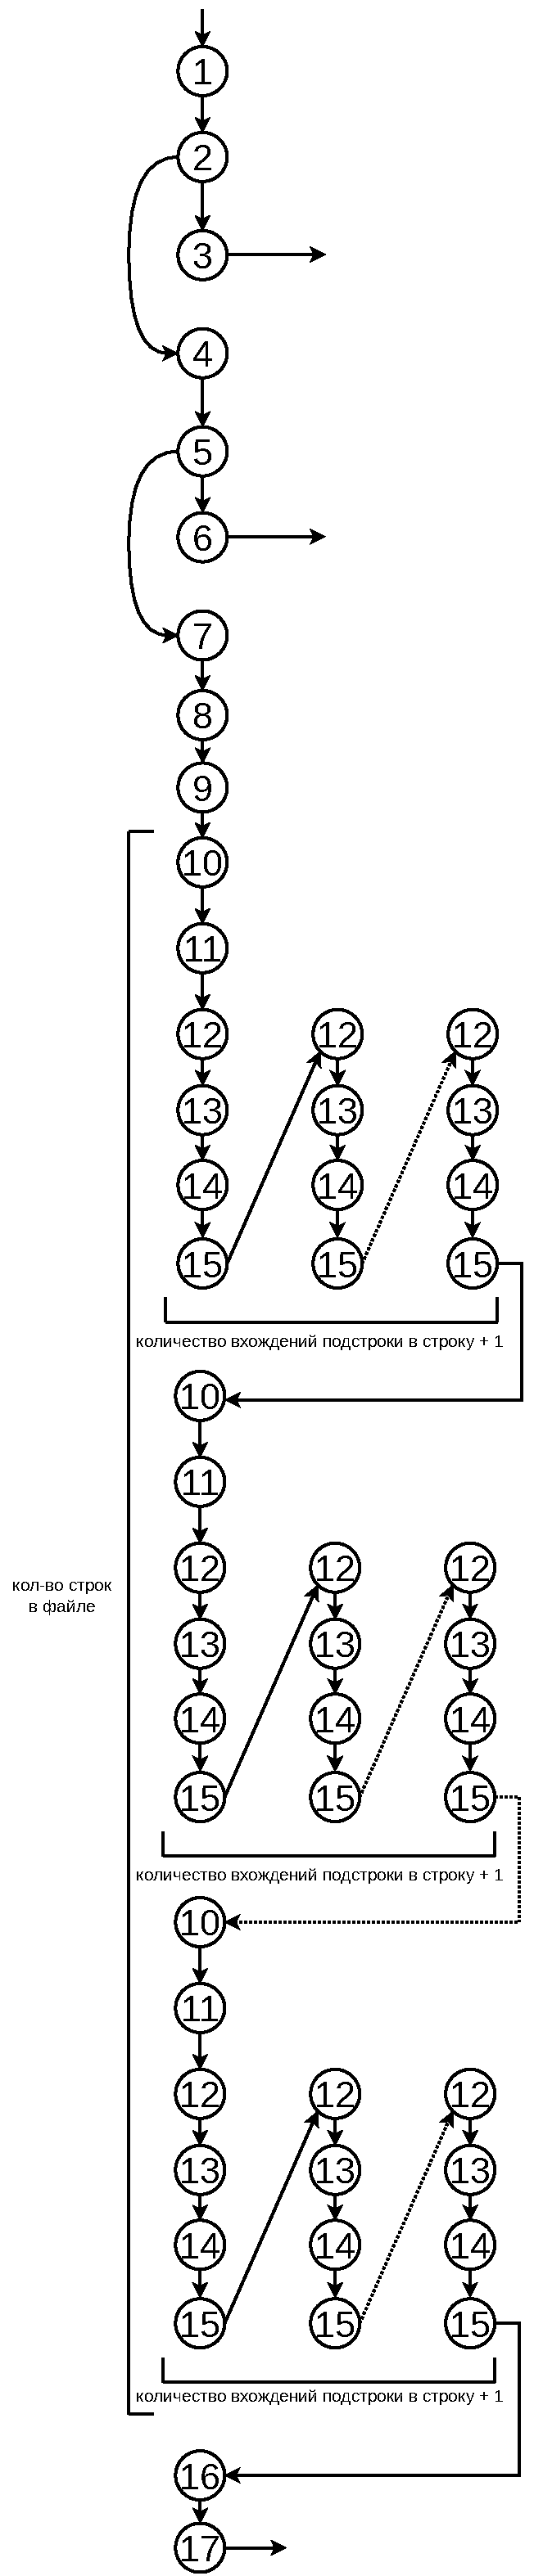
\includegraphics[height=0.95\textheight]{img/ОИ.pdf}
	\caption{Операционная история}
	\label{fig:g3}
\end{figure}

\begin{figure}[h]
	\centering
	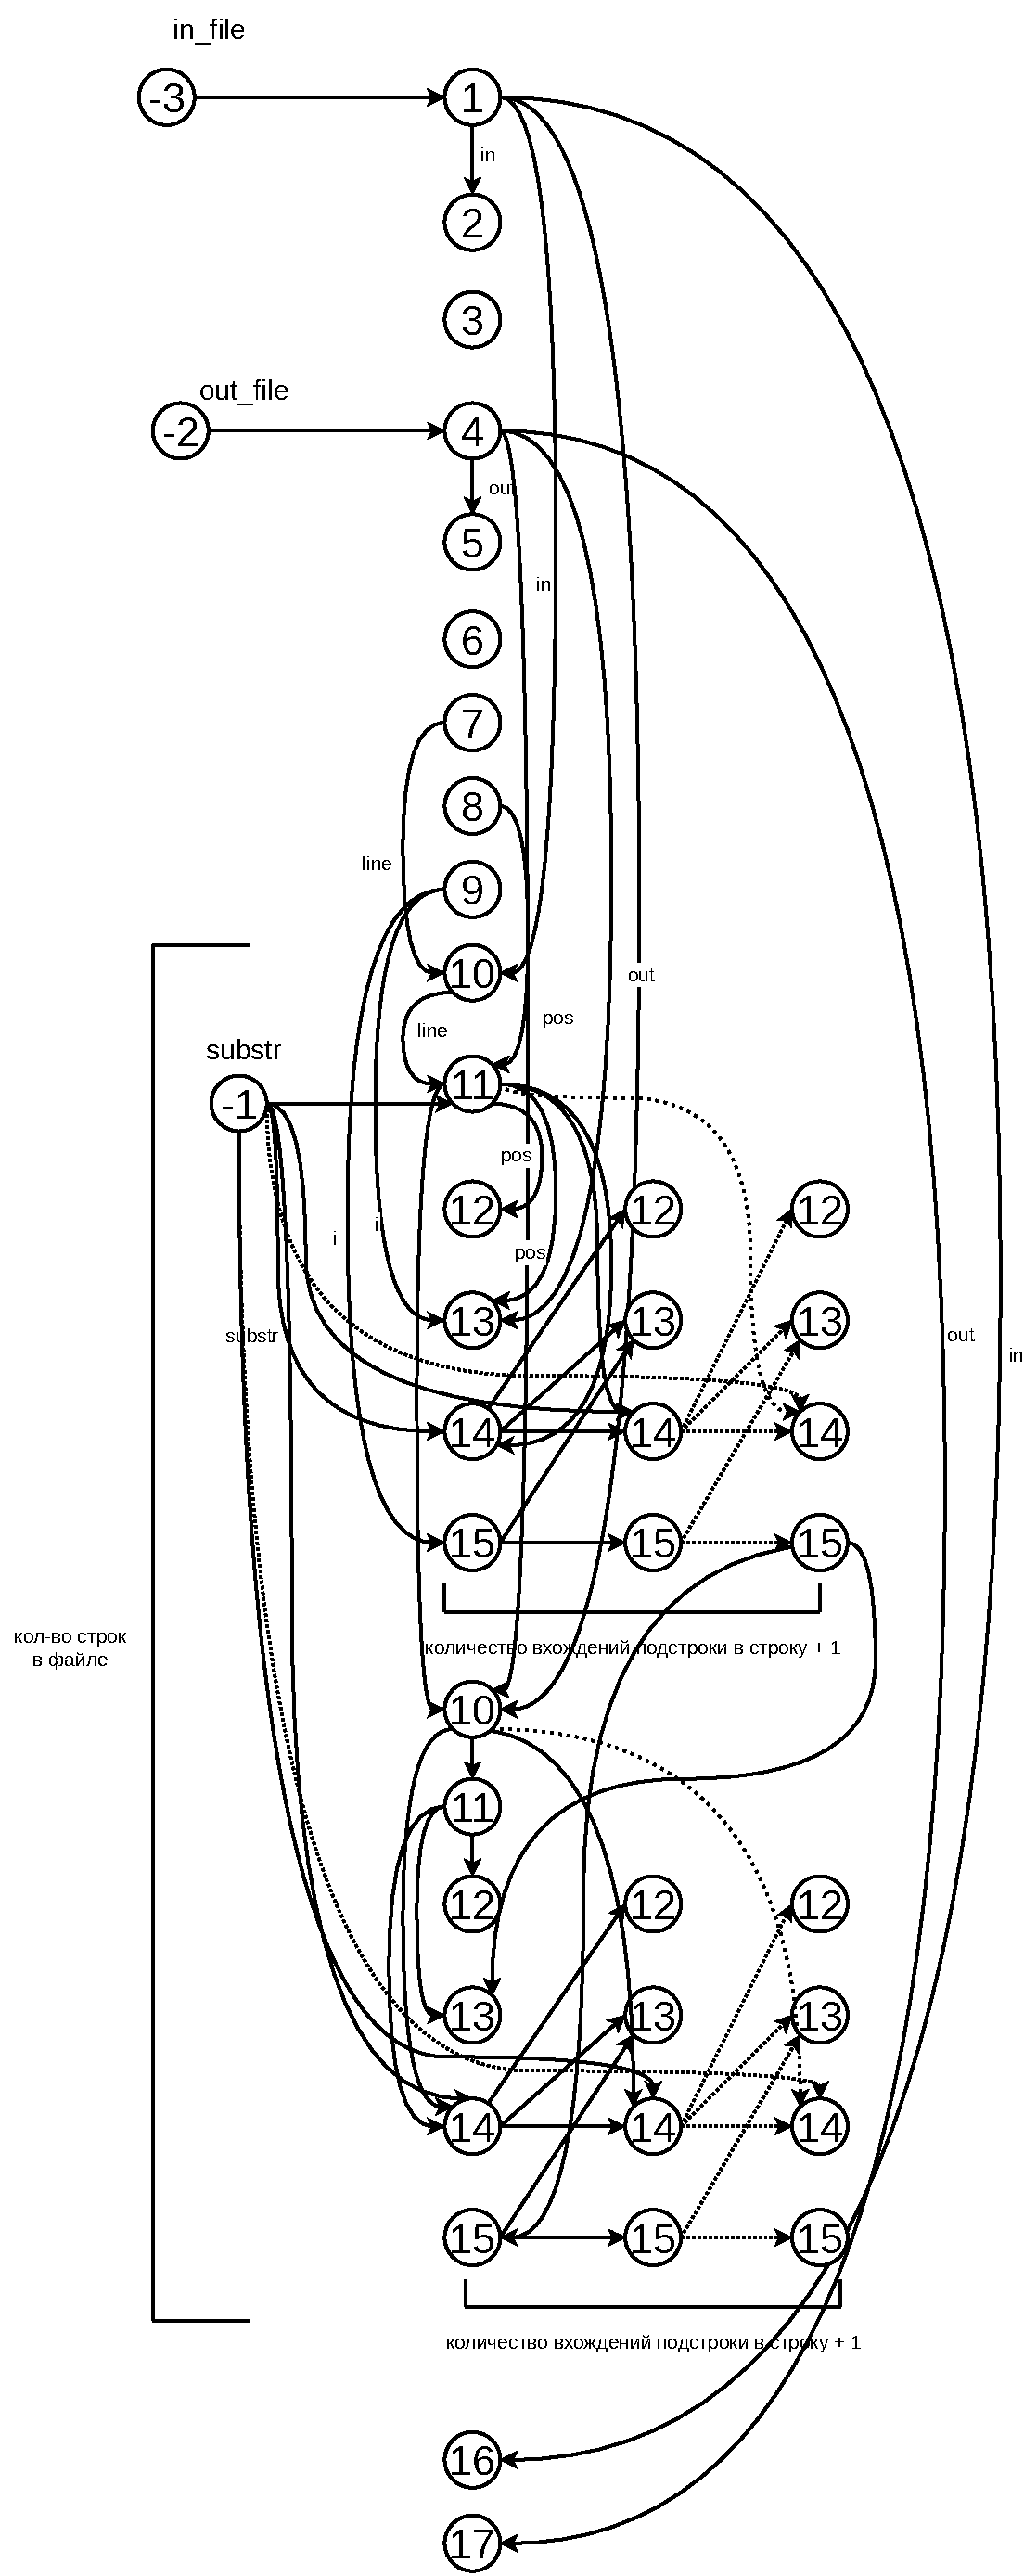
\includegraphics[height=0.95\textheight]{img/ИИ.pdf}
	\caption{Информационная история}
	\label{fig:g34}
\end{figure}

\section{Возможность распараллеливания}

Алгоритм поиска подстроки в файле можно распараллелить, выделив 3 вида потоков:
\begin{itemize}
    \item поток-читатель --- последовательно читает строки из файла;
    \item поток-обработчик --- получает одну из прочитанных строк и находит все вхождения подстроки в неё;
    \item поток-писатель --- получает результаты обработки и записывает их в результирующий файл.
\end{itemize}
